% 5. Présentez votre travail et vos éventuels résultats.
\begin{frame}{Travail réalisé}
  \textbf{Modèle}
  \begin{itemize}
      \item[\checkmark] Intervalles de $\mathbb C$ cartésiens \& polaires
      \item[\checkmark] Diagrammes
      \item[\checkmark] Approximation locale, globale
      \item[\checkmark] Fusion forcée
      \item[\checkmark] Algorithmes de réduction
  \end{itemize}
\end{frame}

\begin{frame}{Modèle théorique}
  \Huge{(Ici, exemple d'un diagramme abstrait additif)}
\end{frame}

\begin{frame}{Modèle théorique}
  \Huge{(Ici, réduction du précédent diagramme)}
\end{frame}

\begin{frame}{Travail réalisé}
  \textbf{Implémentation}
  \begin{itemize}
      \item[\checkmark] Intervalles de $\mathbb C$ cartésiens \& polaires
      \item[\checkmark] Diagrammes : construction, évaluation
      \item[\checkmark] Diagrammes aléatoires
      \item[\checkmark] Fusion forcée
      \item[$\sim$] Algorithmes de réduction
  \end{itemize}
\end{frame}

\begin{frame}{Résultats}
  \begin{columns}
      \begin{column}{0.6\textwidth}
          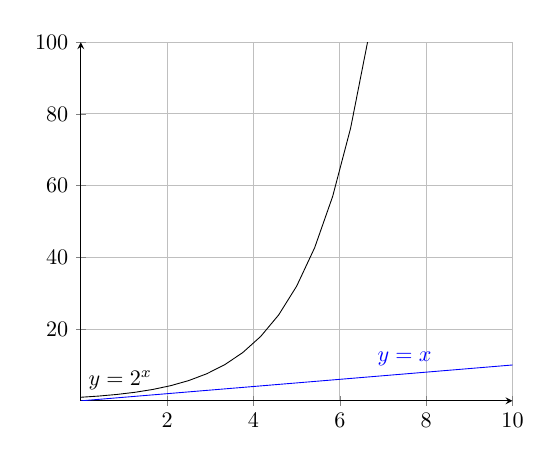
\begin{tikzpicture}[scale=0.8]
              \begin{axis}[grid=both,
                          xmin=0,ymin=0,
                        xmax=10, ymax=100,
                        axis lines=middle,
                        domain=0:10
                        ]
              \addplot[blue]  {x} node[near end, above]{$y=x$};
              \addplot[black]  {2^x} node[at start, above right]{$y=2^x$};
              \end{axis}
          \end{tikzpicture}
              \end{column}
      \begin{column}{0.4\textwidth}
          L'avantage en nombre de nœuds est \textbf{exponentiel} pour le \textit{proof of concept}
      \end{column}
  \end{columns}
\end{frame}
